% Minimal TikZ standalone example
\documentclass[tikz, border=1mm]{standalone}

\usepackage{amsmath}
\usepackage{tikz}

\usetikzlibrary{calc,angles,quotes}

\begin{document}

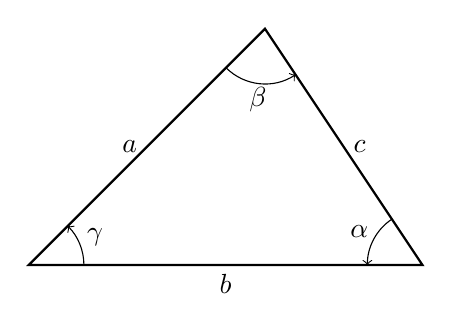
\begin{tikzpicture}[scale=1.0]

	% Points
	\coordinate (A) at (0,0);
	\coordinate (C) at (5,0);
	\coordinate (B) at (3,3);

	% Triangle sides
	\draw[thick] (A) -- (B) -- (C) -- cycle;

	% Side labels
	\node[left]  at ($(A)!0.5!(B)$) {$a$};
	\node[below] at ($(A)!0.5!(C)$) {$b$};
	\node[right] at ($(B)!0.5!(C)$) {$c$};

	% Angle alpha
	\pic[draw, ->, "$\alpha$", angle eccentricity=1.3, angle radius=0.7cm]
	{angle = B--C--A};

	% Angle beta
	\pic[draw, ->, "$\beta$", angle eccentricity=1.3, angle radius=0.7cm]
	{angle = A--B--C};

	% Angle gamma
	\pic[draw, ->, "$\gamma$", angle eccentricity=1.3, angle radius=0.7cm]
	{angle = C--A--B};
\end{tikzpicture}

\end{document}
